% !TEX encoding = UTF-8 Unicode
% !TEX spellcheck = en_US

\documentclass[
	graybox,
	vecphys] % vectors bold face italic (vec command)
	{svmult}

\usepackage{type1cm}        % activate if the above 3 fonts are
                            % not available on your system
%
\usepackage{makeidx}         % allows index generation
\usepackage{graphicx}        % standard LaTeX graphics tool
                             % when including figure files
                             
\graphicspath{{./figures/}}
\usepackage{multicol}        % used for the two-column index
\usepackage[bottom]{footmisc}% places footnotes at page bottom

%%% custom commands
\newcommand{\bm}[1]{\boldsymbol{#1}}
\newcommand{\ks}[1]{{(\mathrm{CS})}_{#1}}
\newcommand{\ortvek}[4]{{ }_{(#1)}{\boldsymbol{#2}}^{#3}_{#4} }
\newcommand{\vek}[3]{\boldsymbol{#1}^{#2}_{#3}}
\newcommand{\trmat}[2]{{{ }^{#1}\boldsymbol{T}}_{#2}}
\newcommand{\rotmat}[2]{{{ }^{#1}\boldsymbol{R}}_{#2}}
\newcommand{\rotmato}[2]{{{ }^{#1}\boldsymbol{\overline{R}}}_{#2}}
% Commands for symbol of the residual (full and reduced)
\newcommand{\Res}[0]{\vec{\delta}}
\newcommand{\ResR}[0]{\vec{\psi}}

%%% custom packages
\usepackage[T1]{fontenc}
\usepackage[utf8]{inputenc}
\usepackage{amsmath,amsfonts}
\usepackage{paralist} % for compactitem
\usepackage{siunitx}
\usepackage{url}
\usepackage{newtxtext}       % 
\usepackage[varvw]{newtxmath}       % selects Times Roman as basic font
\makeindex 

\begin{document}

\title*{Structural and Dimensional Synthesis of Overconstraint Symmetric 3T2R Parallel Robots using Tait-Bryan-Angle Kinematic Constraints}
\author{Moritz Schappler}
\institute{%
Leibniz University Hannover, Institute of Mechatronic Systems. \email{moritz.schappler@imes.uni-hannover.de}. Code: \url{github.com/SchapplM/robotics-paper_ark2022_3T2R}.}

%%% Provide shorter versions of title or author list if neceesary:
 \titlerunning{Synthesis of Overconstraint 3T2R Parallel Manipulators, Tait-Bryan-Angle Kinematics}
 \authorrunning{M. Schappler}

\maketitle
\vspace{-2.5cm} % space above is reserved for author affiliations. Take the space since the one affiliation is on the footer
\abstract{% 10-15 lines long
%Structural synthesis and analysis have shown the characteristics of symmetric parallel robots with three translational and two rotational degrees of freedom (3T2R).
The basic parallel robotics principle of defining kinematic constraints using vector loops is transferred from the general 3T3R case to the 3T2R case by applying a nonlinear Tait-Bryan-angle rotation constraint using the intrinsic $Z$-$Y$-$X$ convention.
This presents an alternative way to the deduction of differential inverse kinematics by the theory of linear transformations.
The resulting formulation is used in a permutational combined structural and dimensional synthesis.
The modular approach allows to combine databases of serial and parallel robots without manual intervention.
The validation shows the reproducability of existing kinematic structures using the new kinematic formulation.
The open-source optimization scheme allows to automatically obtain suitably dimensioned symmetric 3T2R parallel robots.% for a given task.% -- either practical or academic.
%, proven by an example.
} 

%%% Please provide a reasonable number of keywords:
\keywords{Parallel robot, Parallel Manipulator, Overconstraint, 3T2R, Kinematic constraints, Tait-Bryan angles, Euler angles, Dimensional synthesis.}

\section{Introduction and State of the Art}
\label{sec:introduction}

%Parallel robots or parallel manipulators (PM) have been an extensive field of study for several decades now, where fundamentals on analysis and synthesis have been widely covered \cite{Merlet2006}.
A special case of parallel robots or manipulators (PMs) are those with five structural degrees of freedom (DoF): three translational and two rotational (3T2R).
These PMs provide an interesting kinematic structure e.g. for machining tasks. % with rotational symmetry.
Symmetric 3T2R PMs with identical limbs were shown to exist rather late \cite{FangTsa2002,HuangLi2003}.
Since then, works on analysis, modeling and synthesis of these types of PMs have increased %, but this type of machine did not leave it's academic niche. %  for applied mathematicians and engineers
% For a summary see e.g. 
\cite{MotevalliZohSoh2010,GallardoAlvaradoAbeIsl2019}.
%Summaries of the state of the art of 3T2R PMs are e.g. contained in \cite{GallardoAlvaradoAbeIsl2019} or \cite{MotevalliZohSoh2010}.
%
%Stand der Forschung:
%
%fundamentals, first works: 
%\begin{itemize}
%\item first work on symmetric parallel robots with 5 DoF \cite{FangTsa2002,HuangLi2003}. Before it was assumend that these do not exist.
%\item fundamental textbooks on structural synthesis of parallel robots \cite{Gogu2006,KongGos2007}
%\item recent sota \cite{GallardoAlvaradoAbeIsl2019}, other extensive sotas: \cite{MotevalliZohSoh2010}
%\end{itemize}
%\cite{KongGos2007} uses virtual chain which is called PPPU=

The \emph{analysis} of symmetric 3T2R PMs can be performed by several methods.
Most prominent is screw theory \cite{FangTsa2002,KongGos2007,MasoulehGosHusWal2011,GallardoAlvaradoAbeIsl2019}, which can be extended by other algebraic and geometric concepts like Grassmann-Cayley algebra and Grassmann geometry \cite{AmineMasCarWen2012} or algebraic geometry (Study parameters and Gröbner bases) \cite{MasoulehGosHusWal2011}.
For 2T3R PMs Lie groups of displacements were used in \cite{LiHuaHer2004}.
The concept of linear transformations presents an approach of less mathematical complexity and has also been used in the context of general 3T2R PMs \cite{Gogu2008} and together with a geometrical analysis \cite{MotevalliZohSoh2010}.
The existing works focus on different aspects like forward kinematics \cite{MasoulehGosHusWal2011},  %MasoulehHusGos2010a
workspace \cite{MasoulehSaaGosTag2010}, singularity analysis \cite{MasoulehGos2011,AmineMasCarWen2012} or compliance modeling \cite{CaoDinYan2017}.

%methods for modeling:
%\begin{itemize}
%\item Grassmann--Cayley algebra and Grassmann geometry \cite{AmineMasCarWen2012}
%\item screw theory \cite{GallardoAlvaradoAbeIsl2019}
%\item linear transformations \cite{Gogu2006},  linear transformation and geometrical
%analysis \cite{MotevalliZohSoh2010}
%\item algebraic geometry (study parameters) \cite{MasoulehGosHusWal2011}
%\end{itemize}

The \emph{synthesis} of this type of PM has been performed by screw theory in combination with a constraint method \cite{HuangLi2003} or a virtual chain approach \cite{KongGos2007}.
In \cite{DingCaoCaiKec2015} screw theory is used for synthesis together with a systematic deduction and naming scheme to build up a database of symmetric and asymmetric PMs.
In \cite{Gogu2008} the synthesis is performed by evolutionary morphology and the theory of linear transformations, which was taken up in similar form in \cite{MotevalliZohSoh2010}.
%
%Prominent symmetric kinematic structures (i.e. with identical limbs) that have been found are the
%5-R\underline{P}UR   \cite{MasoulehGosHusWal2011,MasoulehGosSaaKon2011,AmineMasCarWen2012,GallardoAlvaradoAbeIsl2019}, the  5-\underline{P}RUR \cite{MasoulehSaaGosTag2010}, 5-RRUR and 5-RPRRR \cite{CaoDinYan2017} or other structures with parallelogram loops \cite{MotevalliZohSoh2010}.
%The established notation denotes prismatic (P) and revolute (R) joints of the parallel kinematic chains counted from the fixed base and marks actuation by underlining \cite{Merlet2006}.
%Other works on non-symmetric PMs, such as the isotropic 3T2R PMs in \cite{Gogu2008} also provide interesting results.
%\end{itemize}
%\begin{itemize}
%\item 5-R\underline{P}UR:  \cite{MasoulehGosHusWal2011,MasoulehGosSaaKon2011,AmineMasCarWen2012,GallardoAlvaradoAbeIsl2019}
%\item 5-\underline{P}RUR: \cite{MasoulehSaaGosTag2010}
%\item 5-RRUR, 5-RPRRR, 5-PRUR \cite{CaoDinYan2017}
%\item with parallelogram loops \cite{MotevalliZohSoh2010}
%\end{itemize}
%
%focus:
%\begin{itemize}
%	\item singularity analysis \cite{AmineMasCarWen2012}
%	\item dimensional synthesis \cite{SongLiaSunDon2014}
%	\item stiffness \cite{CaoDinYan2017}
%\end{itemize}
%
%In summary modeling approaches for 3T2R PMs exist, but are of high mathematical complexity.
Works on robot synthesis give high focus on the \emph{structural} synthesis of the leg chains and mainly provide rules for the synthesis of complete PMs together with some selected examples.
%The works focus on structural synthesis in general and in the analysis of specific aspects.
However, the performance of parallel robots is strongly depending on the \emph{dimensioning} of the parameters \cite{Merlet2006}.

To obtain PMs for a given purpose --- even for an academic example --- the \emph{dimensional} synthesis has to be performed --- either manually or automatically.
Therefore, the structural synthesis should be \emph{combined} with a dimensional synthesis \cite{FrindtKreHes2010}.
The kinematics parameter optimization of a five-DoF PM with complex kinematic structure but few parameters is performed in  \cite{SongLiaSunDon2014}.
Other works on dimensional synthesis like \cite{FrindtKreHes2010} focus on different architectures, but are also transferable to the 3T2R case. %this does not influence the overall principle.
%Dimensional optimization shows good performance when using global multi-objective methods such as a modified form of the strength Pareto evolutionary algorithm \cite{FrindtKreHes2010} or the nondominated sorting genetic algorithm \cite{SongLiaSunDon2014}.

%In many cases the structural synthesis of PMs is performed by manual enumeration.
%Especially when a suitable PM has to be selected for a detailed construction, a database approach like \cite{DingCaoCaiKec2015} allows to shift the focus to the actual design of the robot to be build.


%To summarize
%\begin{compactitem}
%\item The modeling approach for 3T2R robots is of high complexity
%\item most works on parallel robot synthesis give high focus on synthesis of the leg chains and mainly give rules for the synthesis of parallel robots
%\item most work on 3T2R robots focuses on structural synthesis in general and analysis of specific aspects. A tool for the dimensional synthesis is not available
%\end{compactitem}


%To encounter the high modeling complexity for 3T2R PMs, the contributions of this paper are
To further the combined synthesis of 3T2R PMs, the paper's contributions are
\begin{compactitem}
\item an alternative approach to the kinematics model of  symmetric 3T2R PMs with a deduction similar to the theory of linear transformations from \cite{Gogu2008},
\item validating the model in an optimization scheme suitable for combined structural and dimensional synthesis of 3T2R parallel robots,
\item an open-source \textsc{Matlab} toolbox for the kinematics model, the structural and dimensional synthesis toolchain and a serial chain and parallel robot database.
%\item the exemplary synthesis and discussion of 3T2R PMs.
\end{compactitem}

The remainder of the paper is structured as follows. Sect.~\ref{sec:model} introduces the kinematic model for symmetric 3T2R parallel robots.
The combined structural and dimensional synthesis of these robots is discussed in Sect.~\ref{sec:synthesis}.
The results of the synthesis are presented in Sect.~\ref{sec:results} and Sect.~\ref{sec:conclusion} concludes the paper.



\section{Inverse Kinematic Model for 3T2R Parallel Robots}
\label{sec:model}


%The following section presents the new kinematics model based on full kinematic constraints equations.
%\begin{compactitem}
%\item constraints equations usually defined on velocity level by screw theory or theory of linear transformations
%\item nonlinear equations on position level allow solving the inverse kinematics directly in a numeric scheme
%\item approaching the kinematics problem from the nonlinear position level provides an interesting transfer to obtain the linear problem on velocity level
%\item the approach requires the formulation using all joint coordinates (active, passive, including coupling joints). For a real application these can be obtained using the appropriate IK algorithms
%\item general approach: No restriction on the type of leg chain kinematics (hybrid leg chains including parallelograms can only be used if their dependent joints are eliminated from the equations)
%\end{compactitem}

The constraints equations for parallel robots are usually defined on or equivalent to the velocity level when using screw theory \cite{KongGos2007} or the theory of linear transformations \cite{Gogu2008}.
The following section presents an inverse kinematics model based on full kinematic constraints equations, which can be seen as an alternative deduction to the latter method.
%For 3T2R PMs the angular velocity constraints have to be chosen matching to the platform DoF.
%If vectors are expressed in the platform frame, the problem arises that not all orientation DoF are defined in the 3T2R case.
Approaching the kinematics problem from the nonlinear position level can avoid difficulties regarding the reference frame of angular velocities.
A method from \cite{SchapplerTapOrt2019} for 3T3R parallel robots with task redundancy for 3T2R tasks is transferred to the case of 3T2R robots without redundancy.
It should be kept in mind that the method is dedicated to a numeric evaluation and only parts of the expressions are derived symbolically.
An elimination of passive joint coordinates or the use for the forward kinematics problem is not feasible with the proposed approach.
This does not present a disadvantage for the combined synthesis or in simulation. %, which does not present a disadvantage for more complex serial chain structures.
%This does not present a major drawback since a fully symbolic evaluation may be too computationally expensive anyway for more complex robot structures, i.e. with many links or containing many kinematics parameters.

%equations for general model for 3T2R parallel robots
%\begin{compactitem}
%\item model from  \cite{SchapplerTapOrt2019} originally created for 3T3R parallel robots used in 3T2R tasks which provides task redundancy of degree one.
%\item parallel robot with $m=5$ leg chains and $n=5$ operational space coordinates of the platform with operational space coordinate $\bm{x}$

%A parallel robot is considered with $m=5$ leg chains and $n=5$ operational space coordinates $\bm{x}$ of the platform.
%\item coordinate frames are used for modeling the robot: parallel robot base frame $\ks{0}$, leg chain $i$ base frame $\ks{A_i}$, leg chain end frame $\ks{C_i}$, corresponding platform coupling frame  $\ks{B_i}$, platform frame $\ks{P}$ and end effector frame $\ks{E}$ attached to the platform. Without loss of generality, $\ks{P}$ and $\ks{E}$ are assumed to be identically. Another frame $\ks{D}$ is the desired frame in the inverse kinematics problem, where $\ks{E}$ corresponds to the actual frame of the end effector.



\begin{figure}[tb]
\input{./figures/kinematic_sketch.pdf_tex}
\caption{Sketch of the kinematics model at the example of the modified 5-R\underline{P}UR image of \cite{MasoulehGos2011}. Full model with all coordinate frames (\textbf{a}), constraints for first leg chain (\textbf{b}) and other leg chains $i{\ne}1$ (\textbf{c})}
\label{fig:kinematic_sketch}
\end{figure}

A set of coordinate systems $\ks{}$, shown in Fig.~\ref{fig:kinematic_sketch},a, is used to model the parallel robot with $m{=}5$ leg chains $n{=}5$ platform DoF, extending the model of \cite{BriotKha2015}.
The robot base frame $\ks{0}$ is fixed regarding the world frame $\ks{W}$.
Each leg chain has a virtual base frame $\ks{A_i}$ and a virtual end frame $\ks{C_i}$.
This allows a modular use of models for serial kinematic leg chains.
The cut joint frames at the platform are $\ks{B_i}$, corresponding to the leg's $\ks{C_i}$.
%Without loss of generality, the platform frame $\ks{P}$ and the end effector frame $\ks{E}$ are assumed to be identically.
%The latter could include a tool transformation.
The desired end effector frame $\ks{D}$ is used in the derivation of the model and $\ks{E}$ corresponds to the actual frame of the end effector.
%\item Geometry parameters of the parallel robot are given by the homogeneous $\mathrm{SE}(3)$ transformation matrices $\trmat{0}{A_i}$ for the base coupling joint frames, $\trmat{P}{B_i}$ for the platform coupling joint frames and $\trmat{P}{E}$ for the end effector (e.g. a tool) on the platform.
Geometric parameters are given by the $\mathrm{SE}(3)$ matrices $\trmat{0}{A_i}$ for the base coupling joint frames, $\trmat{P}{B_i}$ for the platform coupling joint frames and $\trmat{P}{E}$ for the (for now neglected) end effector (e.g. tool) frame on the platform.

%\item the operational space translational component $\bm{x}_{\mathrm{r}}=\ortvek{0}{r}{}{D}$ is the vector to the desired end effector frame relative to the base frame.
%\item the rotational component marks the pointing direction of the end effector frame using the two angles $\bm{x}_{\mathrm{r}}^\transp=[\varphi_x,\varphi_y]$. Using Cardan angles for the full orientation of the end effector frame gives $\rotmat{0}{D} = \bm{R}_x(\varphi_x) \bm{R}_y(\varphi_y) \bm{R}_z(\varphi_z)$. The third angle $\varphi_z$ corresponds to a rotation around the $z$-axis of $\ks{E}$ and is a dependent variable for robots with five DoF and is therefore not included in the minimal coordinate $\bm{x}$
The translational component of the operational space $\bm{x}_{\mathrm{t}}{=}\ortvek{0}{r}{}{D}$ is the vector to the desired end effector frame relative to the base frame.
The rotational component marks the pointing direction of the end effector frame with the two angles $\bm{x}_{\mathrm{r}}^\transp{=}[\varphi_x,\varphi_y]$.
Using Cardan angles for the full orientation of the end effector frame gives the $\mathrm{SO(3)}$ rotation matrix $\rotmat{0}{D} {=} \bm{R}_x(\varphi_x) \bm{R}_y(\varphi_y) \bm{R}_z(\varphi_z)$.
The third angle $\varphi_z$ corresponds to a rotation around the $Z$-axis of $\ks{E}$ and --- as a dependent variable for 3T2R PMs --- is not included in the five-DoF minimal coordinate $\bm{x}^\transp=[\bm{x}_\mathrm{t}^\transp,\bm{x}_\mathrm{r}^\transp]$.

%=
%\begin{bmatrix}\bm{x}_{\mathrm{t}}^\transp & \bm{x}_{\mathrm{r}}^\transp
%\end{bmatrix}^\transp
%\in {\mathbb{R}}^{5}$

%\item forward kinematics for the first leg chain $i=1$ is defined as $\trmat{0}{E}(\bm{q}_i)=\trmat{0}{A_i} \trmat{A_i}{C_i}(\bm{q}_i)  \trmat{C_i}{B_i} \trmat{B_i}{E}$ % $\ortvek{0}{r}{}{E}(\bm{q}_i) = \ortvek{0}{r}{}{A_i} + \ortvek{0}{r}{}{A_iC_i}(\bm{q}_i) + \rotmat{0}{C_i}(\bm{q}_i) \ortvek{B_i}{r}{}{E}$ 
%setting $\ks{C_i}=\ks{B_i}$, i.e. $\trmat{C_i}{B_i}=\bm{I}$ and with $\trmat{B_i}{E}=\trmat{P}{B_i}^{-1} \trmat{P}{E}$. All joint coordinates of leg $i$ are stacked in $\bm{q}_i$, including all active and passive joints.
The forward kinematics for a leg chain with joint coordinates $\bm{q}_i$ are defined as
\begin{equation}
\trmat{0}{E_i}(\bm{q}_i)=\trmat{0}{A_i} \trmat{A_i}{C_i}(\bm{q}_i)  \trmat{C_i}{B_i} \trmat{B_i}{E}.
\label{eq:fkine_leg}
\end{equation}
% $\ortvek{0}{r}{}{E}(\bm{q}_i) = \ortvek{0}{r}{}{A_i} + \ortvek{0}{r}{}{A_iC_i}(\bm{q}_i) + \rotmat{0}{C_i}(\bm{q}_i) \ortvek{B_i}{r}{}{E}$ 
%setting $\ks{C_i}=\ks{B_i}$
%
The kinematic constraints for the first leg chain $i{=}1$ are expressed as residual regarding $\ks{E}$ from chain 1 and the desired platform frame $\ks{D}$, giving
\begin{equation}
\Res_{\mathrm{t},i}(\bm{q}_i,\bm{x})
=
- \ortvek{0}{r}{}{D,E}(\bm{q}_i,\bm{x})
=
- \bm{x}_{\mathrm{t}} + \ortvek{0}{r}{}{E_i}(\bm{q}_i) \in {\mathbb{R}}^{3}
\label{eq:phi_trans}
\end{equation}
for translation, as depicted in Fig.~\ref{fig:kinematic_sketch},b.
%The vector is expressed in the base frame $\ks{0}$.
The rotational part is
\begin{equation}
\Res_{\mathrm{r},i}(\bm{q}_i,\bm{x})
=
\begin{bmatrix}
\alpha_y & \alpha_x
\end{bmatrix}^\transp
=
\bm{\alpha}_\mathrm{red}\left(\rotmat{D}{E_i}(\bm{x},\bm{q}_i)\right)
=
\bm{\alpha}_\mathrm{red}\left(\rotmat{0}{D}^\transp (\bm{x}_{\mathrm{r}})\rotmat{0}{E_i}(\bm{q}_i)\right) \in {\mathbb{R}}^{2}.
\label{eq:phi1_rot}
\end{equation}
The function $\bm{\alpha}(\bm{R})$ computes the intrinsic $Z$-$Y$-$X$ Tait-Bryan angles $[\alpha_z,\alpha_y,\alpha_x]$ from the given rotation matrix $\bm{R}$ and $\bm{\alpha}_\mathrm{red}(\bm{R})$ does the same and neglects the $Z$ angle.
%\begin{equation}
%\bm{\alpha}(\bm{R}):\mathrm{SO(3)}\rightarrow \mathbb{R}^3
%\quad \mathrm{and} \quad
%\bm{\alpha}_\mathrm{red}(\bm{R})=\begin{bmatrix}
%0 & 1 & 0 \\
%0 & 0 & 1
%\end{bmatrix}\bm{\alpha}(\bm{R}).
%\end{equation}
This nonlinear function allows a minimal coordinate representation of the inverse kinematics problem of 3T2R robots (or tasks) and is not dependent on the uncontrollable (or redundant) variable $\varphi_z$, as elaborated in more detail in \cite{SchapplerTapOrt2019}.

%The second and further leg chains are modeled as following the first leg chain, see e.g. \cite{Gogu2008,BriotKha2015} for similar approaches. %  without reference to the platform frame
The rotational constraints of further leg chains are modeled following the first leg chain. 
See e.g. \cite{Gogu2008,BriotKha2015} for similar approaches on velocity level.
As sketched in Fig.~\ref{fig:kinematic_sketch},c, this is expressed relative to the first leg's rotation matrix $\rotmat{0}{E_1}(\bm{q}_1)$ from (\ref{eq:fkine_leg}) as
%The constraints are
\begin{equation}
\Res_{\mathrm{r},i}(\bm{q}_i,\bm{q}_1)
=
\bm{\alpha}\left(\rotmat{0}{E_1}^\mathrm{T}(\bm{q}_1)\rotmat{0}{E_i}(\bm{q}_i)\right) \in {\mathbb{R}}^{3}
\quad \mathrm{for} \quad i=2,...,m.
\end{equation}
%See also Fig.~\ref{fig:kinematic_sketch},c.
The translational component for further leg chains is linear and therefore used identically as in (\ref{eq:phi_trans}).
The constraints $\Res_i$ for each leg chain and $\Res$ for the full robot are
\vspace{-0.2cm}
\begin{equation}
\Res_i^\transp=\begin{bmatrix}
\Res_{\mathrm{t},i}^\transp & \Res_{\mathrm{r},i}^\transp
\end{bmatrix}
\quad \mathrm{and} \quad
\Res^\transp
=
\begin{bmatrix}
\Res_1^\transp &
\Res_2^\transp &
\cdots &
\Res_m^\transp
\end{bmatrix}.
\label{eq:constr}
\end{equation}
%
A symmetric 3T2R PM 
%each leg chain has $n_i{=}5$ joint DoF and 
has $n_{\bm{q}}{=}25$ active and passive joint DoFs and
the constraints are $\Res(\bm{q},\bm{x}){=}\bm{0} \in {\mathbb{R}}^{29}$, which descriptively shows the overconstraint of degree four.

%The rotation $\varphi_z$ around the end effector $Z$ axis takes a value depending on $\bm{x}$ and the structural parameters of the robot and does not influence the calculation above -- neither does it occur in any way.
%around the end effector $Z$ axis sets as given by the structure of the robot
%
The first-order inverse kinematics can be obtained by partial derivatives as
%of the constraints w.r.t. the joint coordinates $\bm{q}$ and the operational space coordinate $\bm{x}$ giving 
\begin{equation}
\frac{\mathrm{d}}{{\mathrm{d}}t} \Res(\bm{q},\bm{x})
=
\Res_{\partial \bm{q}} \dot{\bm{q}}
+
\Res_{\partial \bm{x}} \dot{\bm{x}}
=
\bm{0}
\quad \mathrm{with} \quad
\Res_{\partial \bm{q}}{:=}\frac{\partial}{\partial \bm{q}} \Res \quad \mathrm{and} \quad \Res_{\partial \bm{x}}{:=}\frac{\partial}{\partial \bm{x}} \Res.
\label{eq:constr_grad}
\end{equation}
%
The gradients in (\ref{eq:constr_grad}) can be obtained in a closed form only depending on known expressions such as the geometric Jacobian of the leg chains and Euler angle transformation matrices \cite{SchapplerTapOrt2019}.
The ``direct kinematic matrix'' \cite{Gogu2008} $\Res_{\partial \bm{q}}$ is rectangular and the linear relation $\dot{\bm{q}}=\tilde{\bm{J}}^{-1} \dot{\bm{x}}$ can be obtained from (\ref{eq:constr_grad}) numerically e.g. using a QR solver.
The tilde sign is used to demarcate the Jacobian corresponding to all joint coordinates (including passive and coupling joints).
For analysis of the robot the (inverse) Jacobian matrix $\bm{J}^{-1}$ corresponding to the active joints $\bm{q}_{\mathrm{a}}$ is needed.
%Fully parallel PMs are assumed with one actuated joint per leg.
The appropriate rows are selected with the matrix $\bm{P}_{\mathrm{a}}$ giving $\bm{q}_{\mathrm{a}} = \bm{P}_{\mathrm{a}} \bm{q}$ and $\bm{J}^{-1}=\bm{P}_{\mathrm{a}} \tilde{\bm{J}}^{-1}$.

This approach has several properties which makes it favorable to use for a combined structural and dimensional synthesis of symmetric 3T2R PMs:

\begin{compactitem}
\item The inverse kinematics problem can be solved using the Newton-Raphson algorithm with $\Res(\bm{q}^{k+1},\bm{x}) {=}
\Res(\bm{q}^{k},\bm{x})
+
\Res_{\partial \bm{q}}(\bm{q},\bm{x}) \rvert_{\bm{q}^k} (\bm{q}^{k+1} {-} \bm{q}^k){=}\bm{0}$ for a step $k$.
\item Only mathematical concepts in the scope of textbooks like \cite{Merlet2006} are necessary, avoiding the explicit use of screw theory and Grassmann or Lie algebra.
\item A completely numeric and modular implementation allows setting up the kinematics model automatically for creation and use of a database of robot structures.
\end{compactitem}

The model (\ref{eq:constr}) has the property of overconstraint, which shows in a rectangular direct kinematic matrix.
This can be avoided by using the reduced orientation residual (\ref{eq:phi1_rot}) on all leg chains.
The geometric elimination of the overconstraint is only permitted if the kinematic constraints can be met, i.e. $\Res{=}\bm{0}$.
This reduced model is written with letter $\ResR$ instead of $\Res$ to easier distinguish the two.
%Now all leg chains use the constraints that was previously only used for the first leading leg chain with unchanged translation $\ResR_{\mathrm{t},i}=\Res_{\mathrm{t},i}$ and rotational part
The translational part stays unchanged with $\ResR_{\mathrm{t},i}=\Res_{\mathrm{t},i}$  and the rotational part is
\vspace{-0.1cm}
\begin{equation}
\ResR_{\mathrm{r},i}(\bm{q}_i,\bm{x})
=
\begin{bmatrix}
\alpha_y & \alpha_x
\end{bmatrix}^\transp
=
\bm{\alpha}_\mathrm{red}\left(\rotmat{D}{E_i}(\bm{x}_{\mathrm{r}},\bm{q}_i)\right) \in \mathbb{R}^2
\quad \mathrm{for} \quad i=1,...,m.
\label{eq:constr_rot_red}
\end{equation}
\vspace{-0.1cm}
The reduced dimension leads to the non-overconstraint $\ResR \in \mathbb{R}^{25}$ and $\ResR_{\partial \bm{q}} \in \mathbb{R}^{25 \times 25}$. % and the formulation is not overconstraint any more.

The Jacobian can be obtained numerically by formulating (\ref{eq:constr_grad}) with $\ResR$ using standard solvers for square matrices like the LU solver.
%
For evaluating the mobility of a parallel robot first the full constraints $\Res$ have to be regarded.
Otherwise a false positive $\ResR{=}\bm{0}$ can result while the full constraints are not met, giving an infeasible $\Res{\ne}\bm{0}$. % and false positive results for valid structures. 
%This is visible by looking at the respective leg chain's forward kinematics $\trmat{0}{E}(\bm{q}_i)$ which gives identical end effector positions $\ortvek{0}{r}{}{E}(\bm{q}_i)$ and pointing directions $\vek{a}{}{D}(\bm{q}_i)$, but different rotation matrices $\rotmat{0}{E}(\bm{q}_i)=[\vek{n}{0}{D}, \vek{o}{0}{D}, \vek{a}{0}{D}]$.}
The leg chain's coupling joints then perform an inconsistent rotation around the end effector's $Z$-axis with feasible $\ortvek{0}{r}{}{E_i}$ and last column in $\rotmat{0}{E_i}$.

\section{Combined Structural and Dimensional Synthesis of 3T2R PMs}
\label{sec:synthesis}

The kinematic model from the previous section is used in a combined structural and dimensional synthesis of symmetric parallel mechanisms (PMs) with 3T2R DoF.
In the \emph{combined synthesis} all possible structures are evaluated by an algorithm which first creates a PM database in a structural synthesis (using the dimensional synthesis implementation) and then performs the dimensional synthesis on the database.
%Instead of using a dedicated structural synthesis, the dimensional synthesis is

%Dimensional synthesis
%\begin{compactitem}
%\item The performance of parallel robots is strongly depending on the kinematic parameters, e.g. the length of the links and the size of the platform \cite{Merlet2006}. This also holds for symmetric 3T2R machines.
%\item For a selection of the best robot for a given task therefore all possible structures should be each optimized independently and then be compared.
%\item Also for academic examples for new kinematic structures a good parameterization helps to show the relevant performance measures.
%\item The dimensional synthesis for a demonstration of the kinematics model for symmetric 3T2R PKM is performed for an exemplary task consisting of consecutive motion in each end effector direction.
%There the kinematic parameters are optimized in a particle swarm optimization (PSO). The whole process is outlined in Fig.~\ref{fig:flowchart_optimization}.
The \emph{dimensional synthesis} is performed for an exemplary task by the kinematics simulation of a representative end effector trajectory. % consecutive motion in each end effector direction.
The kinematic parameters are optimized in a particle swarm optimization (PSO).
The whole process is outlined in Fig.~\ref{fig:flowchart_optimization}.
%For this, a dimensional synthesis has to be performed
The fitness function $\bm{f}$ for evaluating a set of dimensional parameters $\bm{p}$ begins with the solution of the first-order inverse kinematics (IK) on position level 
%using the Newton-Raphson scheme by finding $\Res(\bm{q}){=}\bm{0}$ 
for reference points in the workspace. 
%As elaborated above, using the reduced constraints $\ResR$ give false positive results for valid robots.
If successful, a second-order inverse kinematics is solved for the trajectory using the Jacobian relation.
%The Jacobian matrix is computed
The process is repeated for all PM's IK configurations that are found numerically.
Within the fitness function evaluation several constraints are checked in a hierarchical manner with decreasing priority, meaning that violation of a constraint leads to the abortion of the evaluation and a penalty corresponding to constraint priority.
%\end{compactitem}
Some of the constraints (checked in structural ``S'' or dimensional ``D'' synthesis) are (in this order)	
\begin{compactitem}
\item[(S/D)] geometric plausibility (e.g. leg chain lengths vs base/platform dimensions), 
\item[(S/D)] success of the inverse kinematics (first and second order), 
\item[(S)] check validity of full kinematic constraints $\Res{=}\bm{0}$,
\item[(D)] self-collisions (with elementary geometry such as spheres and capsules), 
\item[(D)] installation space (e.g. robot has to be in a cylinder with reasonable radius),
\item[(D)] joint angle ranges and velocities (to be in a technically feasible range of values).
\end{compactitem}
%The letters S/D denote whether a constraint is checked in dimensional (D) or structural synthesis (S).
%If all constraints are met, the feasible robot is evaluated regarding performance criteria such as condition number of the Jacobian $\bm{J}$ and the length of the leg chains.


%If the dimensional synthesis is performed for all possible robot structures, it can be termed ``combined structural and dimensional synthesis''.

\begin{figure}[b!]
\vspace{-0.4cm} % to keep image on page with beginning of Sect. 3
\centering
\input{./figures/optimization_flowchart.pdf_tex}
\caption{Overall procedure for the dimensional synthesis of a robot with hierarchical constraints}
\label{fig:flowchart_optimization}
\end{figure}

\pagebreak

In the \emph{structural synthesis} mode of the toolchain 
% the last three constraints are ignored and
the objective is to obtain the mobility based on the Jacobian $\bm{J}$.
%
%Structural synthesis
% For numbers of the robot structures see parrob_mdlbib/examples_tests/number_of_robots_in_database.m
%
By this framework there is no need of a complex geometric analysis as done by other authors.
The underlying assumption is that a numeric evaluation of the PM mobility is possible if (and only if) the kinematic constraints can be met.
%
%
%\begin{compactitem}
%\item The kinematics model presented in this paper is used for a structural synthesis of symmetric parallel robots with five degrees of freedom
%\item This presents a foundation for the following dimensional synthesis which is also used as a framework for the validation of structures.
%\item general approach is similar to \cite{Gogu2008}
While many implementation details are different, the general leg chain synthesis approach is similar to \cite{Gogu2008} and the database approach is similar to \cite{DingCaoCaiKec2015}.
Serial kinematic leg chains are obtained by permutation of Denavit-Hartenberg parameters and successive elimination of isomorphisms which leaves 213 possible serial kinematic leg chains with five joints consisting of revolute (R) or prismatic (P) joints.
Substituting some RR-subchains with universal (U) joints further gives 180 variants.
The geometric characteristics of possible symmetric parallel robots is obtained from literature.
%(see Sec.~\ref{sec:introduction}) 
This leads to several possible joint alignments relative to the fixed base (transformation $\trmat{0}{A_i}$) or the moving platform (transformation $\trmat{P}{B_i}$). % which mainly regards the alignment of the $z$-axis as the joint axis in DH notation.
The synthesis is performed by permutation of all implemented possibilities for leg chain, base coupling, platform coupling and actuation with additional filtering for feasibility (e.g. no passive prismatic joints, proximal actuation). % and by running the dimensional synthesis for each PM candidate.
%\begin{compactitem}
%\end{compactitem}
Eleven PMs with four joints (classes 5-PRUR, 5-RPUR, 5-RRUR, 5-RUPR, 5-RURR) and 16 PMs with five joints (classes 5-PRRRR, 5-RPRRR, 5-RRPRR, 5-RRRRR) are generated.

\section{Exemplary Results of the Combined Synthesis for 3T2R PMs}
\label{sec:results}

These structures are validated for an exemplary task with middle position of $[r_{\mathrm{T}x},r_{\mathrm{T}y},r_{\mathrm{T}z}]{=}\bm{x}^\transp_\mathrm{T,t}{=}[0,0,\SI{1500}{\milli\metre}]$ in the world frame.
%
%
The tilting angles $[\varphi_{\mathrm{T}x},\varphi_{\mathrm{T}y}]{=}\\\bm{x}^\transp_\mathrm{T,r}{=}[\SI{20}{\degree},\SI{20}{\degree}]$ of the tool axis have to be non-zero to avoid singularities.
The end effector pose is then changed consecutively by $\pm$\SI{300}{\milli\metre} for each position component of $\bm{x}_\mathrm{t}$ and $\pm$\SI{10}{\degree} for the orientation $\bm{x}_\mathrm{r}$. % $\varDelta r_x{=}\pm$\SI{42}{\milli\metre}, $\varDelta r_y{=}\pm$\SI{42}{\milli\metre} and $\Delta r_z{=}\pm$\SI{42}{\milli\metre} \varDelta \varphi_x{=}\pm$\SI{42}{\degree} and  $\varDelta \varphi_y{=}\pm$\SI{42}{\degree}
The parallel mechanism is floor-mounted and the base position $\bm{r}_0^\transp{=}[r_{0x},r_{0y},r_{0z}]$ is subject to optimization with  $\SI{-600}{\milli\metre}{<}r_{0x},r_{0y}{<}\SI{600}{\milli\metre}$ and $\SI{0}{\milli\metre}{<}r_{0z}{<}\SI{800}{\milli\metre}$.
The base diameter is allowed to be  $\SI{1400}{\milli\metre}{<}d_\mathrm{B}{<}\SI{3000}{\milli\metre}$ and the platform diameter to be $\SI{200}{\milli\metre}{<}d_\mathrm{P}{<}\SI{800}{\milli\metre}$.
Further one scaling parameter, one platform coupling joint alignment angle parameter and one to seven Denavit-Hartenberg parameters \cite{BriotKha2015} are subject to the optimization, leading to nine to 15 parameters in total, depending on the kinematic structure of the robot. 
The high number of dimensional parameters facilitates finding a non-singular setting of the robot. % but requires an algorithm with good exploration capabilities like multi objective PSO.
%Singularities hinder the practical use of parallel robots in general and the demonstration of academic examples for symmetric 3T2R PMs in particular.
%
Minimization objectives in the multi-objective PSO are the condition number and the summed lengths of the leg chains as indicators for general feasibility.
The optimization with up to 200 generations and 100 individuals took \SI{7}{\hour} to \SI{10}{\hour} per robot on a state-of-the-art Intel Xeon computing cluster system, running in parallel using a \textsc{Matlab} implementation (with time limit of \SI{10}{\hour}).

The results are summarized in a Pareto diagram shown in Fig.~\ref{fig:results},a.
%
%\begin{figure}[tb]
%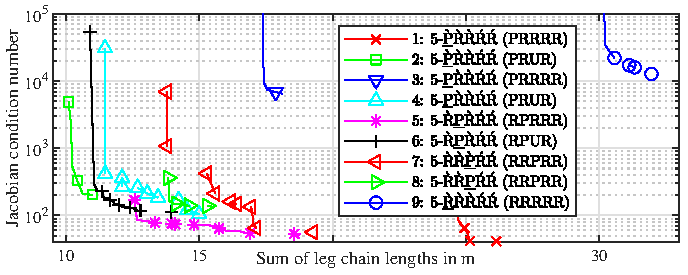
\includegraphics{pareto_all.pdf}
%\caption{Results of the exemplary optimization}
%\label{fig:pareto}
%\end{figure}
%
The robots in Fig.~\ref{fig:results},b are named using the established PM notation \cite{Merlet2006} together with the kinematic chain notation from \cite{KongGos2007}, where joints with the same accent on \`R or \'R are parallel to each other and underlined \underline{R} or \underline{P} are actuated.
In addition, \underline{\`P}\`R and \underline{\'P}\'R subchains are used to distinguish the structures as this provides more information than \underline{C} in \cite{MasoulehSaaGosTag2010}.
% for actuated parallel kinematic machines. %and Fig.~\ref{fig:robots3} for parallel kinematic chains without regard of the actuation.

\begin{figure}[tb]
\centering
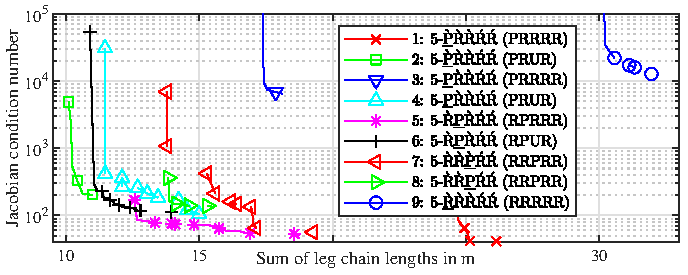
\includegraphics{pareto_all.pdf}
\input{./figures/robots.pdf_tex}
\caption{Results of the synthesis: Pareto front  \textbf{(a)}, robot examples in $\bm{x}_\mathrm{T}$ \textbf{(b)} with active prismatic base coupling joint (numbers 1--4), and with revolute base joint and active prismatic joint (no. 5--8)}
\label{fig:results}
\end{figure}

Known structures like the 5-R\underline{P}UR (no.~6) \cite{MasoulehGosHusWal2011,AmineMasCarWen2012,GallardoAlvaradoAbeIsl2019} and 5-\underline{P}RUR (no.~4) \cite{MasoulehSaaGosTag2010} can be reproduced.
The 5-{\`R}\underline{P}{\`R}{\'R}{\'R} (no.~5) emerges when separating the DoF of the universal joint of no.~6.
The same goes for no.~3 emerging from no.~4.
Structures like this may not be popular in literature due to the higher number of kinematic parameters, difficulty of analysis and the necessity of the dimensional synthesis beyond manual parameter tuning.
Some structures are unconventional like 5-\underline{\`P}{\`R}{\`R}{\'R}{\'R} (no.~1 and 2) similar to the \underline{C}UR chains of the Pentapteron in \cite{MasoulehSaaGosTag2010}.
Structure no.~7 is disadvantageous for technical realization due to the distal position of the actuation in the chain, despite its acceptable performance.
Robots with only revolute joints like the 5-RRUR reported in \cite{CaoDinYan2017} were not successful due to self collisions with the long limbs required for the large-scale platform motion as can be seen by high values for no. 9 in the Pareto diagram.


%\begin{figure}[tb]
%TODO
%%\input{./figures/robots2.pdf_tex}
%\caption{Example of robots with only revolute joints. The actuation for full mobility requires an active joint in distal parts of the leg chains, making them unfavorable for technical realization.}
%\label{fig:robots3}
%\end{figure}

\section{Conclusion}
\label{sec:conclusion}
% Layout: This section should start on the last page
\vspace{-0.1cm} % for conclusion section to start on page 8

The presented inverse kinematics model for 3T2R PMs can be regarded as a variation of the theory of linear transformations.
%The level of mathematic complexity 
%and necessary knowledge on advanced geometry or algebra 
%is lower than for other methods.
%This is bought dearly by a higher number of variables, which on the upside allows generalization.
Using the model in a combined structural and dimensional synthesis allows to reproduce relevant symmetric 3T2R parallel robots. % without the necessity of manually analyzing specific robots.
%The results can be used for further investigations on the robots and for eventually finding new interesting structures.
The practical application of symmetric 3T2R robots will be promoted by the open-source \textsc{Matlab} tool which generates feasible dimensioned robot structures. % for given task parameters.

\vspace{-0.3cm}
\begin{acknowledgement}
The author acknowledges the support by the Deutsche Forschungsgemeinschaft (DFG) under grant number 341489206. \textsc{Matlab} code to reproduce the results
is available at GitHub under free license at \url{github.com/SchapplM/robotics-paper_ark2022_3T2R}.
%
\end{acknowledgement}

\vspace{-0.5cm}
\bibliographystyle{spmpsci}
\bibliography{references}

\end{document}
